%% the problem?
What is a mathematical model of attack trees?  There have been
numerous proposed answers to this question.  Some examples are
propositional logic, multisets, directed acyclic graphs, source sink
graphs (or parallel-series pomsets), Petri nets, and Markov processes.
Is there a unifying foundation in common to each of these proposed
models?  Furthermore, can this unifying foundation be used to further
the field of attack trees and build new tools for conducting threat
analysis?

The answer to the first question is positive, but the answer to the
second question is open.  Each of the proposed models listed above
have something in common.  They can all be modeled in some form of a
symmetric monoidal category
\cite{Tzouvaras:1998,Brown:1991,Fiore:2013,FrancescoAlbasini2010}.
That is all well and good, but what can we gain from monoidal
categories?

Monoidal categories are a mathematical model of linear logic as
observed through the beautiful Curry-Howard-Lambek correspondence
\cite{Mellies:2009}.  In linear logic every hypothesis must be used
exactly once, and hence, if we view a hypothesis as a resource, then
this property can be stated as every resource must be consumed.  This
linearity property is achieved by restricting the logic so that
hypothesis are never duplicated or removed.

Multisets and Petri nets both capture the idea that the nodes of an
attack tree consist of the attack action and the state -- the
resource -- of the system being analyzed. As it turns out, linear
logic has been shown to be a logical foundation for multisets
\cite{Tzouvaras:1998} and Petri Nets \cite{Brown:1991}.  Thus, linear
logic has the ability to model the state as well as attack actions of
the goals of an attack tree.  

In this paper\footnote{This material is based upon work supported by
  the National Science Foundation CRII CISE Research Initiation grant,
  ``CRII:SHF: A New Foundation for Attack Trees Based on Monoidal
  Categories``, under Grant No. 1565557.} I introduce a new logical
foundation of attack trees -- with and without costs -- in linear
logic; the type of attack trees considered in this paper are attack
trees with sequential conjunction due to Jhawar et
al.~\cite{Jhawar:2015}.  This new foundation is based on a new logic
called the Attack Tree Linear Logic (ATLL).

\begin{wrapfigure}{r}{0.5\textwidth}
  \vspace{-30px}
  \begin{center}
    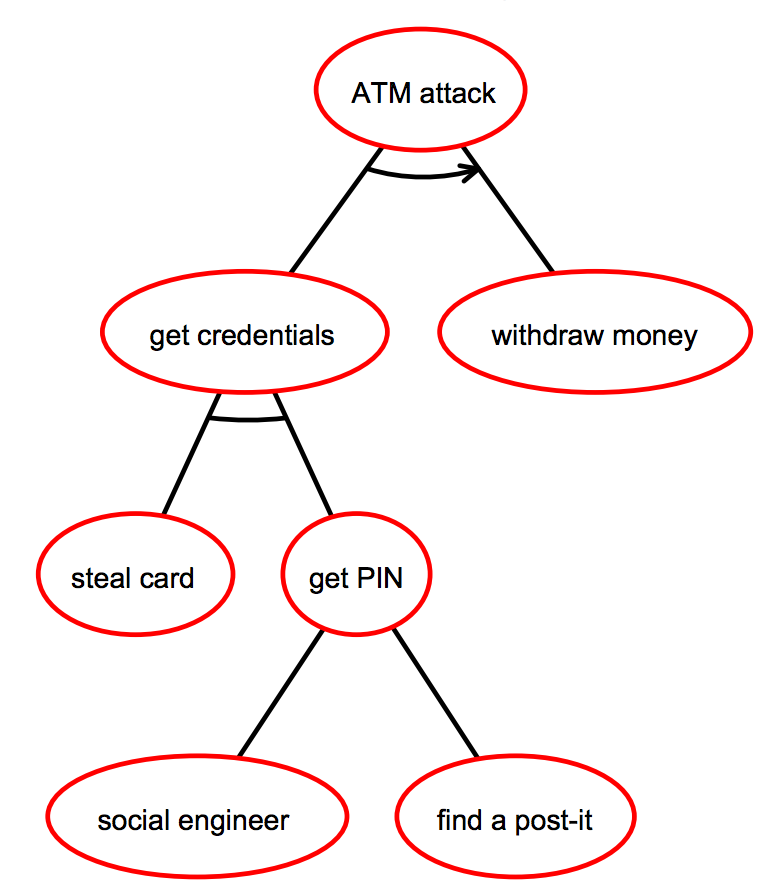
\includegraphics[scale=0.225]{ATM-Tree1}
  \end{center}  
  \label{fig:atm-tree1}
  \caption{Attack Tree for an ATM attack from Figure~1 on page 2 of Kordy et al.~\cite{Kordy2017}}
  \vspace{-55px}
\end{wrapfigure}
In ATLL (Section~\ref{sec:attack_trees_without_costs}) attack trees
are modeled as linear formulas where base attacks are atomic formulas,
and each branching node corresponds to a binary logical connective.
Consider the attack tree for an ATM attack from
Figure~\ref{fig:atm-tree1}.  We can model this attack tree as a
formula in ATLL as follows:
\[
\begin{array}{lll}
  [[B1]] := \text{``steal card''}\\
  [[B2]] := \text{``social engineer''}\\
  [[B3]] := \text{``find a post-it''}\\
  [[B4]] := \text{``withdrawal money''}\\
  [[T1]] := [[(B1 (.) (B2 + B3)) > B4]]
\end{array}
\]
Each $[[Bi]]$ is an atomic formula, parallel conjunction of attack
trees is denoted by $[[T1 (.) T2]]$, choice between attacks by $[[T1 +
    T2]]$, and sequential conjunction of attacks by $[[T1 > T2]]$.
Parallel conjunction and choice are both symmetric, but sequential
conjunction is not.  Now that we can model attack trees as formulas we
should be able to use the logic to reason about attack trees.

Reasoning about attack trees corresponds to proving implications
between attack trees.  In fact, every equation from Jhawar et al.'s
work on attack trees with sequential conjunction \cite{Jhawar:2015}
can be proven as an implication in ATLL.  Consider a second attack
tree from Figure~\ref{fig:atm-tree2}.
\begin{figure}
  \begin{center}
    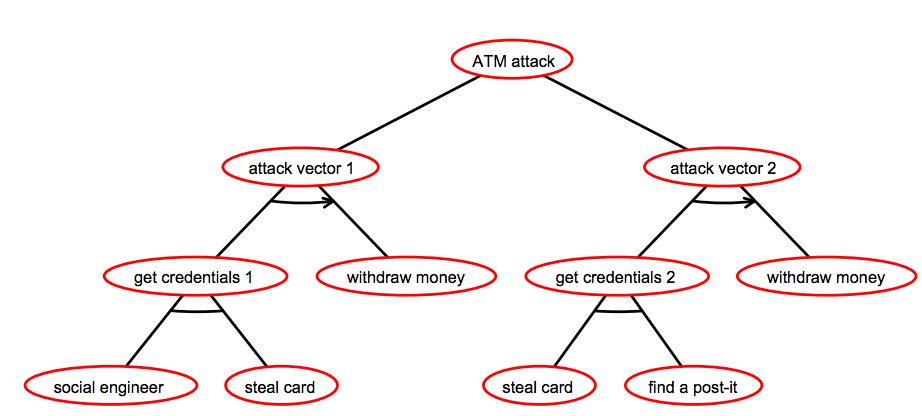
\includegraphics[scale=0.35]{ATM-Tree2}
  \end{center}
  \caption{Canonical Attack Tree for an ATM attack from Figure~2 on page 3 of Kordy et al.~\cite{Kordy2017}}
  \label{fig:atm-tree2}
\end{figure}
We can model this attack tree as a formula in ATLL as well (the base
attacks are the same):
\[
\begin{array}{lll}
  [[T2]] := [[((B1 (.) B2) > B4) + ((B1 (.) B3) > B4)]]
\end{array}
\]
The attack trees $[[T1]]$ and $[[T2]]$ represents the same attack, and
this can be proven in ATLL by showing that $[[T1 o-o T2]]$ where
$[[o-o]]$ denotes bi-implication.  The proof holds by using the
distributive rules for choice.

In addition, implication can be used to prove subattack tree
relationships between attack trees.  For example, supposed we wanted
to show that the tree $[[B1 (.) B2]]$ is a subattack tree of $[[T2]]$,
then this is the case if $[[T2 -o (B1 (.) B2)]]$. This requires some
additional rules be added to ATLL and this is discussed in
Section~\ref{sec:attack_trees_without_costs}.

Using a generalization of Bucciarelli and
Ehrhard’s~\cite{BUCCIARELLI:2000} indexed linear logic I extend ATLL
with costs.  I call this extension Indexed ATLL
(Section~\ref{sec:attack_trees_with_costs}).  In this system every
base attack is annotated with a cost, and every branching node is
associated with a binary operation used for computing the cost at that
node.  Then implication is associated with a binary relation on costs.
This new binary relation is used to insure that the costs of two trees
are related when proving implications between attack trees.  Thus, one
can prove facts about attack trees in Indexed ATLL that require one to
reason about both the tree structure as well the quantitative data in
the tree simultaneously.

Modeling attack trees in linear logic has a number of benefits.
First, it connects attack trees back to logic, but in elegant and
simple way.  Kordy et al.~\cite{Kordy2010,Kordy:2012} proposed that
attack trees be modeled in propositional logic, but in this model
attacks can be freely duplicated and contracted which goes against the
process/resources nature of an attack tree.  However, linear logic
restores this natural interpretation without loosing the process
interpretation of attack trees and without having to resort to
complicated notion unlike models similar to the situation calculus
\cite{Samarji2013}.  By connecting attack trees to logic we can also
tap into the long standing research and development of automation, for
example, SAT, SMT, proof search, etc.  Finally, by connecting to logic
we also connect to the theory of statically typed functional
programming through the Curry-Howard-Lambek correspondence which will
allow for the development of a programming language that can be used
to certify the correctness of attack trees and the analysis performed
using them.

\textbf{Contributions.}  This paper offers the following
contributions:
\begin{itemize}
\item The Attack Tree Linear Logic (ATLL): a new linear logic for the
  specification and analysis of attack trees.
\item The Indexed Attack Tree Linear Logic (Indexed ATLL): an
  extension of ATLL with costs and the ability to reason about them
  while reasoning about attack trees.
\item A few new and interesting open problems.
\end{itemize}
